\section{Introduction}
During the last years the usage of smart-wearables (particularly smartwatches) has become more and more common with a number of 337 million units sold in 2019 and a forecast in sales of up to 527 million units by 2024 \cite{tenzer}.
With that also comes a natural demand in data protection due to the many sensors built in these devices due to their ability to capture sensible personal information (e.g. health informations) and additionally the fact that smart devices also can now be used for many kinds of financial actions.
Since most wearables are connected to either the distributors or the respective mobile phones virtual assistant they should contain sensors for on one hand sound conduction and on the other hand audio recording.
Based on these conditions smartwatches could be used in combination with biometric authentication mechanics.
\newline
Previous works in this field exploited amongst others gyro- and acceleration-sensors for the purpose of authentication \cite{johnston2015smartwatch}, \cite{yang2015motionauth}.
Based on these results it is arguable that there is room for smartwatch based authentication. Also with the presentation of a novel kind of biometrics named \textit{functional biometrics} the use of smart wearables as a medium for implicit and passive authentication rises.
\newline
Focussing on these new techniques this work introduces a prototype for smartwatch based authentication using body conduction of sound. This prototype can be classified in the category of functional biometrics. It uses a microcontroller equipped with a microphone and speaker to generate and capture an audio sample.

\section{Related Work}
In general biometric authentication can be split into behavioural and physiological biometrics as well as authentication can be split into implicit and explicit methods.
The exact characteristics will be described as follows: 
\subsection{Biometrics}
\textit{Biometrics} (as in the greek terms \textit{bios} and \textit{metrikos}) describes the utilization of an individuals physical traits or behaviour to clearly identify one from others. Contrary to the more known verification methods as PINs, passwords or ID-cards biometric identification does not rely on tokens or knowledge which could easily be forgotten or stolen, rather than unique personal traits like fingerprints, face or the specific way someone interacts \cite[chpt. 1.1]{jain2007handbook}\cite{delac2004survey}.
Therefore the individual wishing to authenticate first has to enrol one specific trait of hers to the biometric system. Based on this sample data the system generates an authentication template which is later on used to authenticate against. 
When someone now wants to register using the system he provides the trait wanted to the system from which then a new sample is generated. The generated sample then is compared to the template \cite{alsaadi2015physiological}.
Tests used for this comparison can be designed based on two different points of view. First of positive identification or authentication and second negative identification/authentication.
Negative authentication presumes the given sample is from an unknown user whereas the sample in a positive authentication scenario should be by a known user \cite{wayman2005introduction}.
As already stated above biometric authentication uses an individuals personal traits as authentication tokens. Based on the kind of trait and the methods how they could be provided the general term of biometrics can be further divided into \textit{behavioural} and \textit{physiological} biometrics. How each of them is defined exactly will be defined in the following.
\subsubsection{Behavioural Biometrics} Behavioural biometrics refers to authentication systems in which process of authentication is conducted with the use of primarily gestures or other actions able to be performed in everyday life.
Usable features for this purpose are e.g. gait or keystroke analysis. Advantages this kind of biometrics has are e.g. that there is no direct need for special hardware since it is mostly used with smart wearables or mobile phones who each have the required sensors built in.
Another advantage would be that the data required must not be collected actively by the user but is recorded passively by the sensors of the used smart device \cite{yampolskiy2008behavioural}.
\subsubsection{Physiological Biometrics} Apart from behavioural biometrics there is also the classification of physiological biometrics.
This form of biometric authentication uses the more "static" traits of a users body as tokens such as e.g. fingerprints, hand geometry, vein patterns \cite{alsaadi2015physiological}, \cite{faltaous2019vpid}.
A physiological system should also have a little higher accuracy than a behavioural one and it should be harder to use as an imposter since it is nearly impossible to identically copy a finger print, iris pattern, etc. \cite{koong2014user}, \cite{delac2004survey}.
\subsubsection{Functional Biometrics} With functional biometrics another novel kind of biometric authentication was introduced lately by Schneegass et al. \cite{schneegass2020functbiometric}.
This new concept stands as a major influence to this work notably with its first implementation in SkullConduct\cite{SkullConduct}. 
\begin{figure}
	\begin{center}
		\subfloat[Traditional Biometrics]{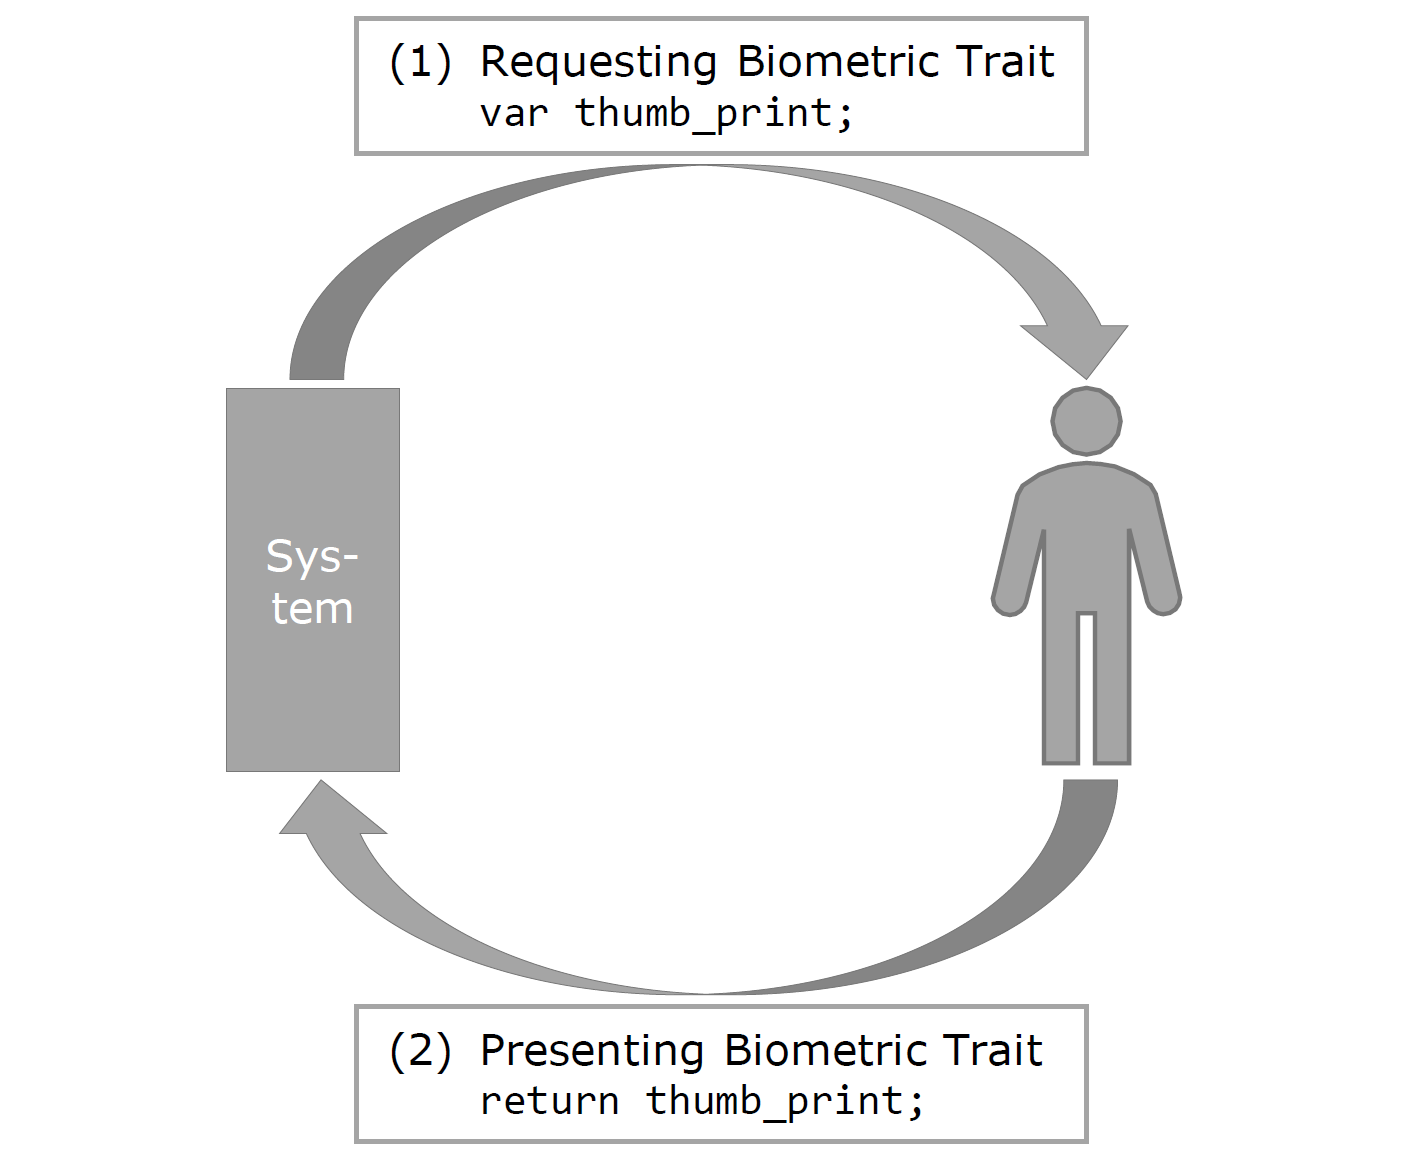
\includegraphics[width=0.4\textwidth]{biometric_trad.png}\label{fig:tradBiom}}
		\hspace{0.5cm}
		\subfloat[Functional Biometrics]{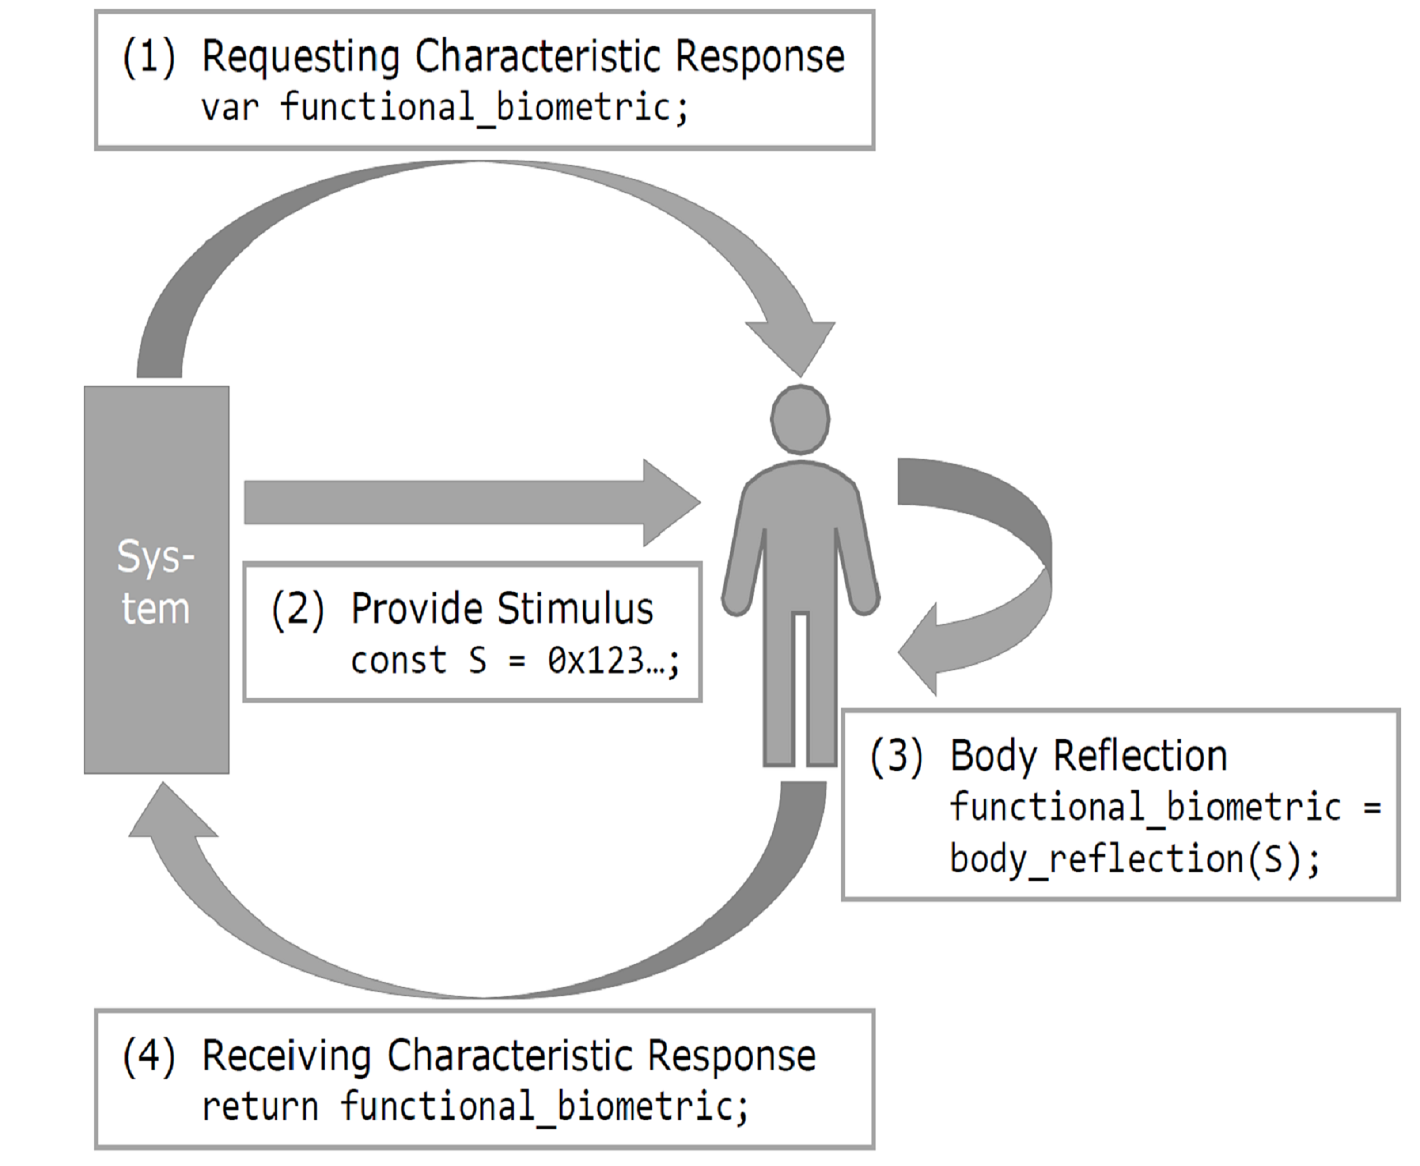
\includegraphics[width=0.4\textwidth]{biometric_funct.png}\label{fig:functBiom}}
	\end{center}
	\caption{Fig.~\ref{fig:tradBiom} shows the authentication process of a traditional biometric system. Fig.~\ref{fig:functBiom} shows the order of steps for functional biometrics when a stimulus is added \cite{schneegass2020functbiometric}.}
	\label{fig:biometricsVersions}
\end{figure}
\newline
In this category of biometric authentication the authentication system provides an additional stimulus during the enrolment phase.
This stimulus is applied to the individuals body where it gets modified and afterwards captured (Figure~\ref{fig:functBiom}).
Due to different personal biological characteristics the modification of the stimulus is unique for each combination of user and stimulus.
Requirements Schneegaß et al. proposed are two hardware components in form of a Stimulus Generation Unit (SGU) and a Body Reflection Sensor (BRS).
These two have to be designed as a dependence of the underlying biometric trait. Exemplarily when sound is used as the stimulus the SGU will be most likely some kind of microphone and the BRS a speaker.
During the enrolment process described above stimulus and its transformation are saved as a secret two-tuple ($x, f(x)$) with $ x $ being the stimulus and $ f(x) $ the transformation.
Now when the related user wants to authenticate the stimulus is reapplied and it is expected to get $f(x)$ as response again.
An additional security measure provided by functional biometrics is that when the stimulus gets leaked or lost the system is not fully compromised because the stimulus is only an exchangeable medium.
The secret stems from the body reflection function which is unique to the user, unknown and hard to manipulate.
\subsection{Authentication} 
A further subdivision which can be made in the context of authentication is between explicit and implicit authentication. By \textit{explicit} authentication one understands interactions with a security system which are performed actively.
This includes providing knowledge like PIN or password, using a token but also performing gestures, fingerprints etc. from the biometrical field. 
Work presented by Shi et al. states that \textit{implicit} authentication would be a perfect fit for usage in combination with mobile devices \cite{shi2010implicit}.
Since users are using their devices on slightly different habits everyday the data collected by built-in sensors alternates between individuals but stays the same for one person.
Exploiting this they propose three application scenarios for the use of implicit authentication.
First as a second factor in combination with passwords, second as the main authenticator and thus replacing the usage of a password and last as additional assurance or an extra trust factor when performing financial actions on a mobile device.

As already mentioned before the SkullConduct work by Schneegass et al. is one of the key influences to this work. Not just because it is one of the first realizations for functional biometrics but it also 
serves as a source of inspiration for this work.
Schneegass et al. implemented a biometric authentication system using eyewear computers (e.g. Google Glass).
Therefore they used the concept of bone conduction which is already frequently used by hearing aids. SkullConduct, in this case, uses the bone conduction speaker of the Google Glass to emit a sound sample against the wearers head.
The sample which gets transformed due to the unique nature of each individuals head is captured by the glasses integrated microphone.
Results of this study  indicate that with all tested users SkullConduct had a probability of around 97\% when it comes just to identify a correct user.
Test of the system as an authentication tool showed an Equal Error Rate (EER) of around 6.9\% in average but with significant drops the shorter the used sample gets (less than 1 second).
\newline
\newline
Other work on authentication via smart devices includes e.g. the works from A. Johnston et al. who implemented a smartwatch based authentication module that used gait recognition \cite{johnston2015smartwatch}.
They adapted from previous work of theirs where gyro- and acceleration-sensors of smart phones were used to develop authentication methods \cite{kwapisz2010cell}.
The main thought behind the proposed use of gait authentication on smartwatches is that their place of wearing/usage is more consistent than the one of a smart phone and therefore more advantageous.
Each participants dataset includes both data from gyro- and acceleration-sensor.
Tests in regard of both design types showed that the general performance of authentication is way higher in average than the one of identification (e.g. 97.2\% compared to 79.2\%).
Additionally the overall performances of the acceleration-sensor was higher than the gyro-sensor.
Conclusions Johnston et al. drew from their results were that it is possible to authenticate someone sufficient enough using a smartwatch but they propose not to use the system for something other than a multi-modal biometric system at its current level. 

\section{Concept}
%In this work a prototype for a smartwatch based authentication tool will be implemented.

%Motivations are that there is a demand in security measures for mobile smart devices (like smartwatches)  
\section{Implementation}
\section{Evaluation}
\section{Conclusion}
